\documentclass[11pt]{article}
\usepackage[margin=1in]{geometry} %
\usepackage{amsmath,amssymb,mathtools} %
\usepackage{hyperref} %
\usepackage{tikz} %
\usepackage{inconsolata} %
\usepackage{listings} %
\usepackage{enumitem} %
\setlist{noitemsep,topsep=2pt} %
\lstset{ %
basicstyle=\ttfamily\small, %
columns=fullflexible, %
keepspaces=true, %
showstringspaces=false, %
frame=single %
} %
\title{idealFlow.cpp and data structures}
\author{Jay}
\date{}
\begin{document}
\maketitle

\section{Overview}
This document explains the structure and logic of the C++ code \texttt{idealFlow.cpp}, which solves 1D ideal hydrodynamics using PETSc. The code reads simulation parameters from a JSON file, sets up the computational grid, initializes the solution, and advances it in time using a finite-volume method, high resulotion scheme.\\

\underline{Note to self: Change diagrams to better ones!}

\begin{itemize}
    \item Charges: $E, M_{x}$
    \item Thermo variables: $p, \, \beta, \, c^2_{s}$
    \item primitive variables: $e,\, u_{x}$
\end{itemize}

\section{Input Handling}
The code reads simulation parameters from a JSON file (default: \texttt{inputs.json}). The relevant parameters include:
\begin{itemize}
    \item \texttt{NX}: Number of grid points
    \item \texttt{xmin}, \texttt{xmax}: Domain boundaries
    \item \texttt{dof:} degrees of freedom per grid point/node, 7 in this case
    \item \texttt{CFL}:
    \item \texttt{iofilename}: Output HDF5 file name
    \item \texttt{initial\_time}, \texttt{final\_time}: Simulation time range
    \item \texttt{steps\_per\_print}: Output frequency
\end{itemize}

\section{Main Data Structures}
\subsection{Class: EOS}
The \texttt{EOS} class encapsulates the equation of state. It provides methods to compute pressure, speed of sound, temperature, and other thermodynamic quantities as functions of energy density $e$ (ignore the baryon density $\rho_B$ for now).

\subsection{Struct: VischydroNode}
This structure represents the hydrodynamic state at a single grid point. Its members (degrees of freedom at each node/grid point) are:
\begin{itemize}
    \item \texttt{E}: Energy
    \item \texttt{M}: Momentum
    \item \texttt{e}: Energy density
    \item \texttt{ux}: Fluid velocity
    \item \texttt{p}: Pressure
    \item \texttt{beta}: Inverse temperature
    \item \texttt{cs2}: Speed of sound squared
\end{itemize}
It also provides methods for computing charges, fluxes, and derived quantities.\\

\begin{figure}[h]
    \centering
    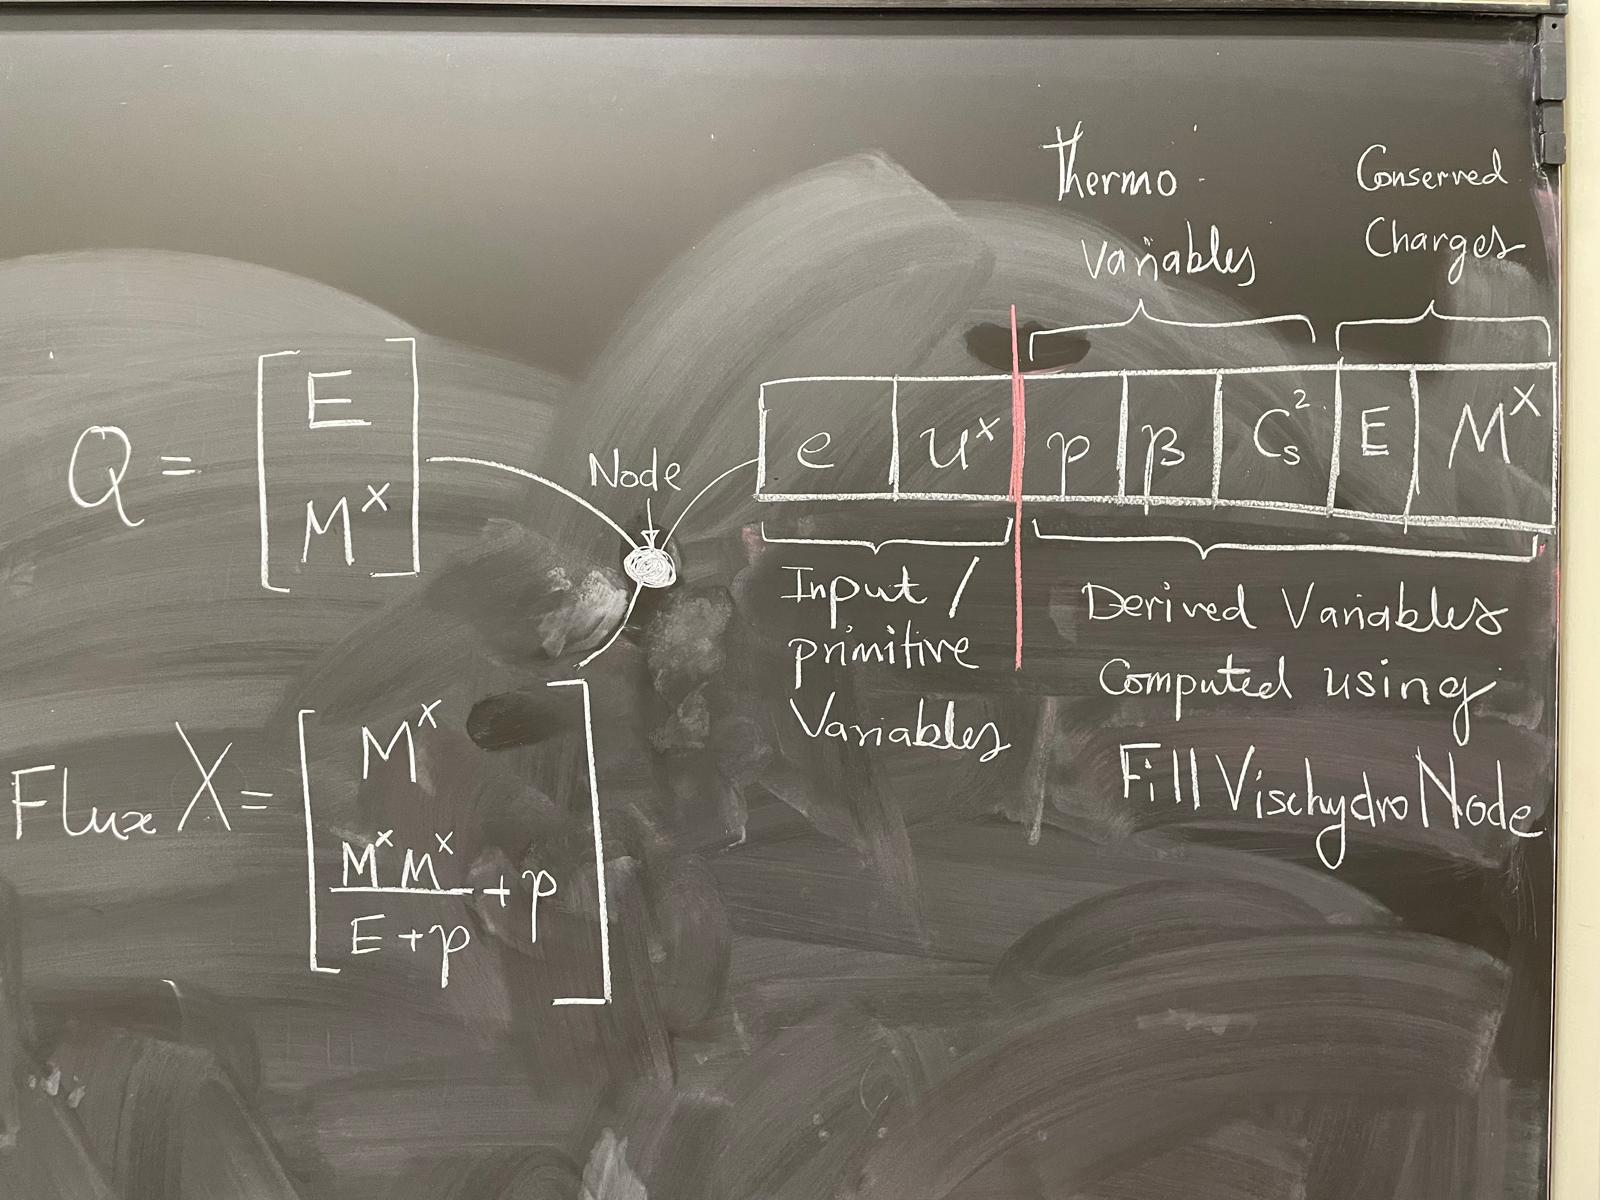
\includegraphics[width=0.8\linewidth]{node.jpeg}
    \caption{schematic diagram of a node and all the data on it}
    \label{fig:node}
\end{figure}


\subsection{Class: Vischydro}
This class manages the entire simulation, including:
\begin{itemize}
    \item Reading inputs
    \item Setting up the PETSc DMDA grid
    \item Initializing solution vectors
    \item Managing the PETSc time stepper (TS)
    \item Outputting results to HDF5
\end{itemize}

\begin{figure}[h]
    \centering
    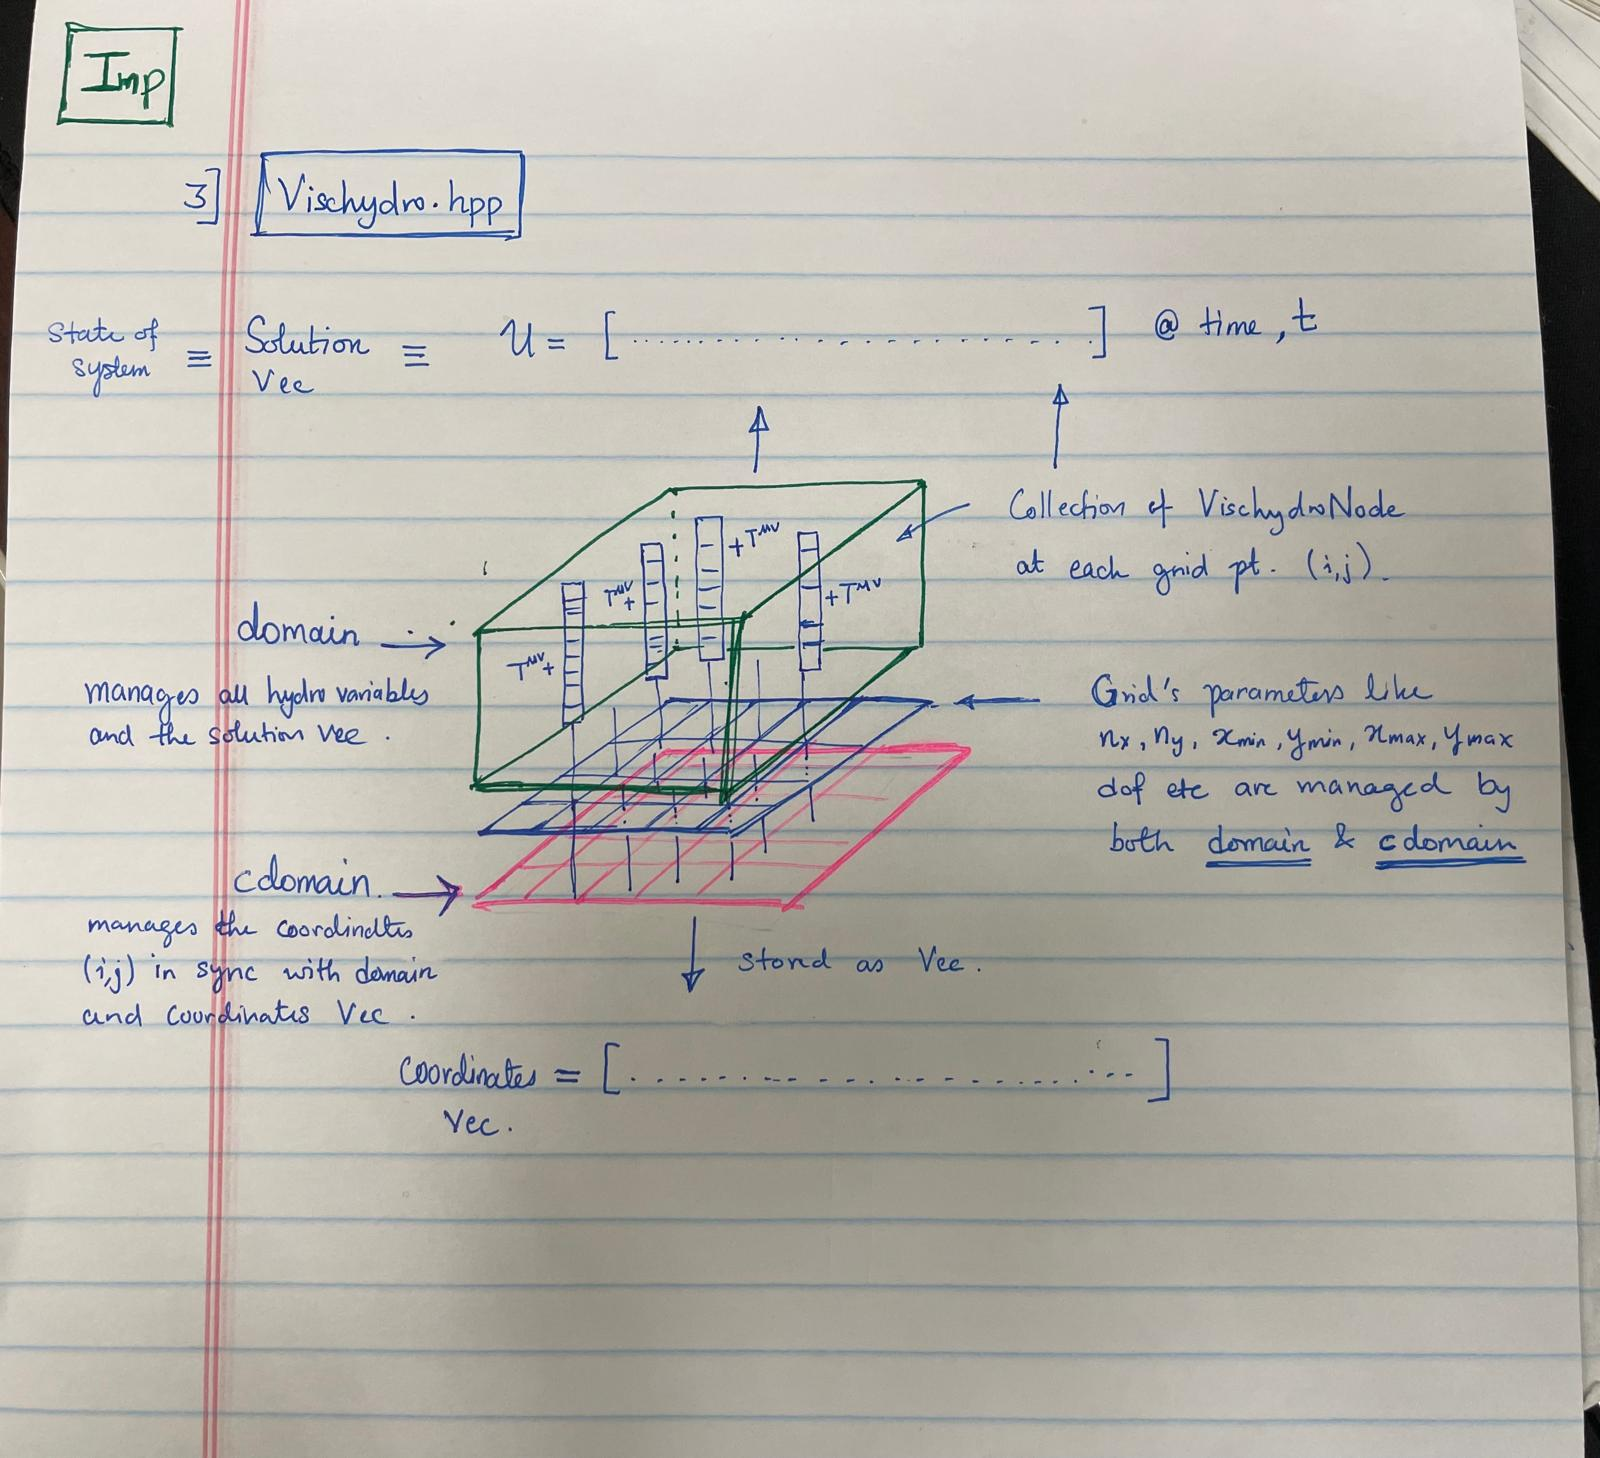
\includegraphics[width=0.8\linewidth]{vischydro.jpeg}
    \caption{Ignore the label `vischydro.hpp' for this case. This is a schematic diagram of how vischydro class is designed}
    \label{fig:vischydro}
\end{figure}


\section{Algorithm}
\begin{enumerate}
    \item \textbf{Initialization}: Read inputs, set up grid, initialize solution with a Gaussian energy profile.
    \item \textbf{Time Stepping}: Advance the solution using PETSc TS. At each step:
    \begin{itemize}
        \item Compute fluxes using a slope limiter and Riemann solver.
        \item Update solution vectors.
        \item Output results at specified intervals.
    \end{itemize}
    \item \textbf{Post-processing}: Write final solution to HDF5.
\end{enumerate}

\section{Helper Functions}
\begin{itemize}
    \item \texttt{FillVischydroNode}: Starting with energy density `$e$' and EOS, this function  fills the VischydroNode with charges $E, M$ and thermo variables $p, \, \beta, \, c^2_{s}$
    \item \texttt{idealHydroCellSolve}: Given $E, M$, using Newton's method, this routine finds the energy density '$e$' and updates thermo variables  $p, \, \beta, \, c^2_{s}$
    \item \texttt{EulerRHSFunction}: Used for \underline{explicit} time-stepping. Computes the fluxes and updates the time derivatives of the conserved quantities for all grid cells, enabling PETSc to advance the hydrodynamic simulation in time.
    \begin{itemize}
        \item Copy take global solution ($U$) $\rightarrow$ local array with ghost cells
        \item using flux limitter and Riemann solver reconstruct the state and flux at each node
        \begin{figure}[h]
            \centering
            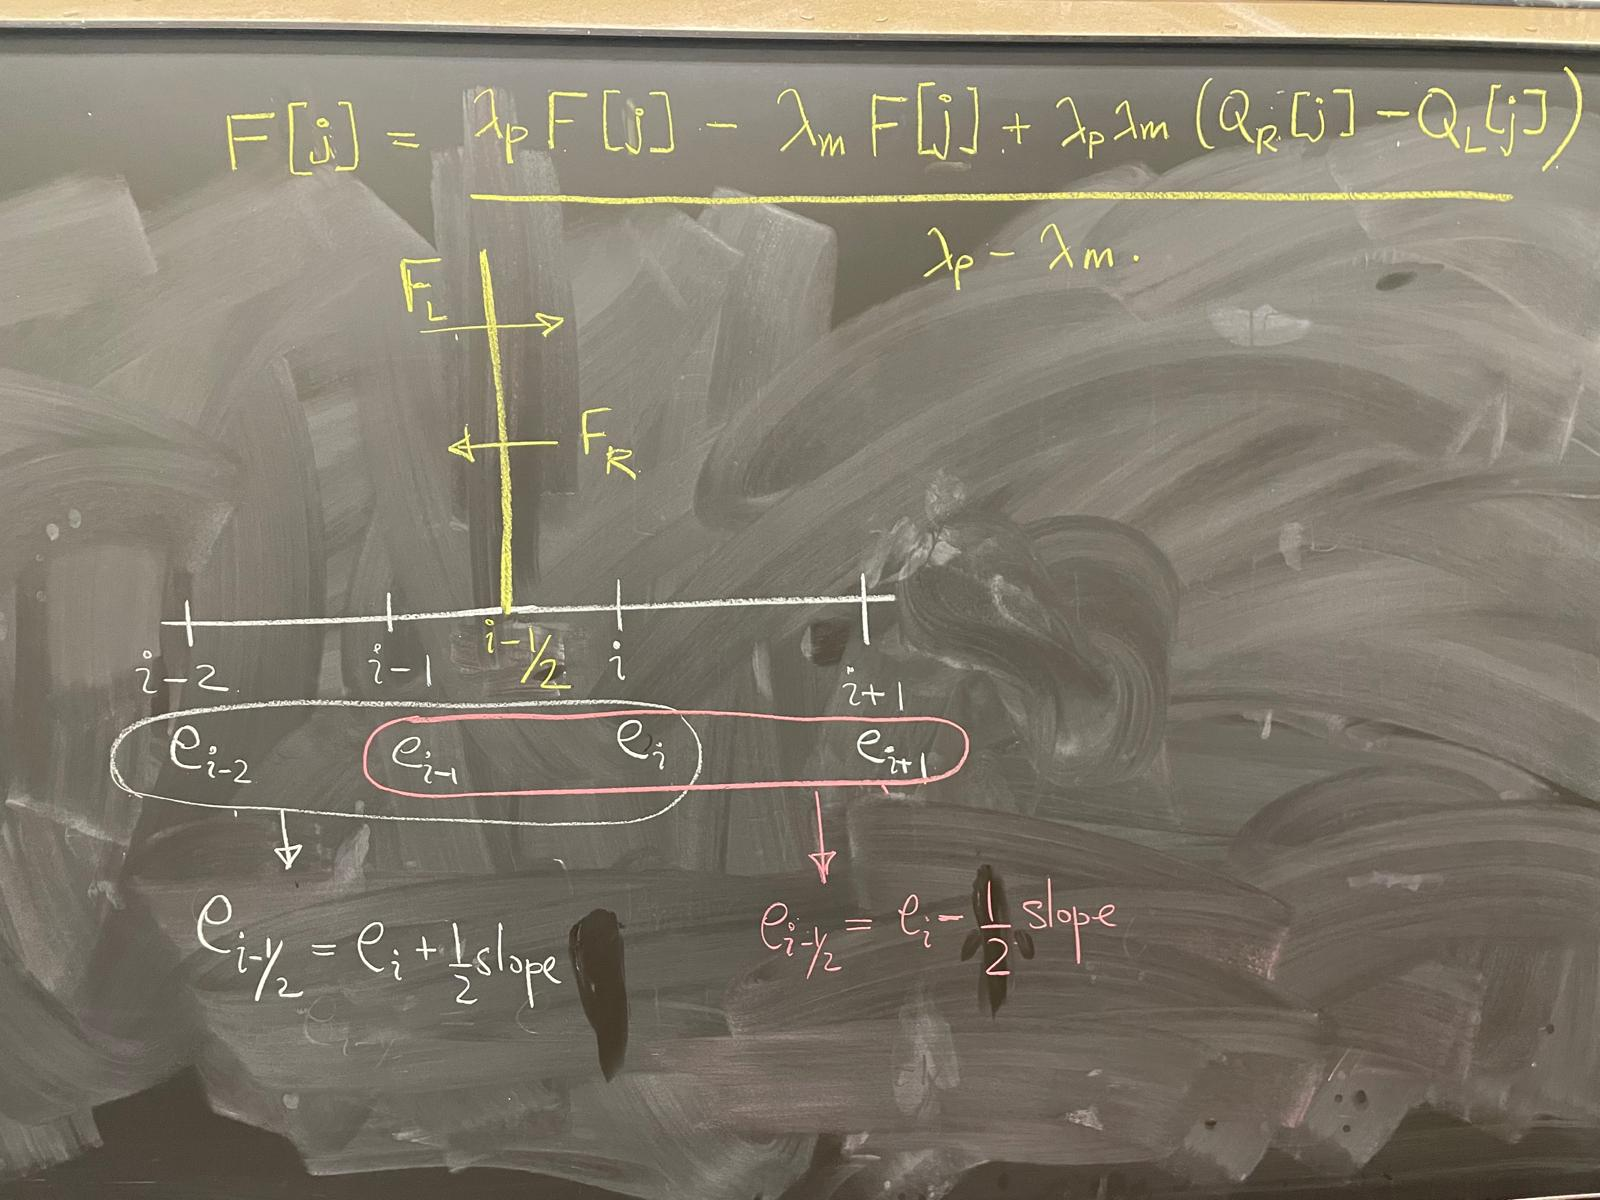
\includegraphics[width=0.8\linewidth]{flux.jpeg}
            \caption{Schematic diagram explaining how energy density $e$ from neighboring grid points is used along with central minmod to calculate $e_{i-1/2}$. This in turn is used to calculate charges and thermo variables, which are then used to calculate the HLL flux shown in yellow. $\lambda_{p/m}$ are the propogation speeds for the flux in plus(p) and minus(m) directions}
            \label{fig:placeholder}
        \end{figure}
        \item Assemble the flux into output vector ($G$) which would represent the time derivative due to the explicit terms (ideal part)
    \end{itemize}
    \item \texttt{VischydroMonitor}: Outputs solution at each time step.
\end{itemize}

\section{Data Flow}
\begin{itemize}
    \item The main solution vector is a PETSc Vec of \texttt{VischydroNode} structs.
    \item At each time step, the solution is updated using fluxes computed from neighboring nodes.
    \item Output is written to an HDF5 file for post-processing and visualization.
\end{itemize}

















\end{document}

